%% IMPORTANT: Once working, run latex 3 times to get listoffigures to work

%% Be sure to check spelling!

%% Put **your** name and the proper due date in place

%% Copy the lstlisting and figure code as many times as you need
%% Be sure to put in your own file names if appropriate

%% Note that the \epsfig command is currently commented out - until the
%%%% files exist, processing this code without them will result in an error
%%%% so leave the comments until you have created the graphics files!

\documentclass{article}
\usepackage{amsmath}    % loads AMS-Math package
\usepackage{epsfig}     % allows PostScript files
\usepackage{listings}   % allows lstlisting environment
\usepackage{moreverb}   % allows listinginput environment
\usepackage[letterpaper, margin=0.75in]{geometry}  % set paper size/margins
\usepackage{textcomp}   % adds \interrobang, among others!

\begin{document}
\begin{center}
\rule{6.5in}{0.5mm}\\~\\
\textbf{\large EGR 103L -- Fall 2017}\\~\\
\textbf{\huge Laboratory 7 - Roots and Extrema}\\~\\
Ian Hanus (ih52)\\
Lab Section 1B, Tuesday 8:30-11:20 AM\\
October 29th, 2017
{\small I understand and have adhered to all the tenets of the Duke
  Community Standard in completing every part of this assignment.  I
  understand that a violation of any part of the Standard on any part
  of this assignment can result in failure of this assignment, failure
  of this course, and/or suspension from Duke University.} 
\rule{6.5in}{0.5mm}\\
\end{center}
\tableofcontents
\listoffigures
\pagebreak

\section{Basic Root-Finding Problems}
\begin{center}
\renewcommand{\arraystretch}{1.5}
\begin{tabular}{|c|c|c|}
\hline Function & Real Roots & Roots\\ \hline
$f(x)= 20e^{-4x}-36e^{-2x}+18e^{-x}-1$ & 3 & 4.5651e-02, 6.3358e-01, 2.7546e+00 \\ \hline
$f(x)= x^5+100\mbox{cos}(2x)$ & 3 & -7.8392e-01, 7.8691e-01, 2.1295e+00\\ \hline
$f(x)=\frac{10}{x-2}-90e^{-(x/2)}$,$x\neq 2$ & 2 & 2.3619e+00, 7.9669e+00\\ \hline
\end{tabular}
\end{center}

\section{Basic Min/Max-Finding Problems}
\begin{center}
\begin{tabular}{|c|c|c|}
\hline Function & Counts & Extrema\\ \hline
$f(x)= 20e^{-4x}-36e^{-2x}+18e^{-x}-1$ & 1 min, 1 max & min:$f(2.4510e-01)=-1.4596e+00$\\
 & & max:$f(1.3002e+00)=1.3421e+00$\\ \hline
$f(x)= x^5+100\mbox{cos}(2x)$ & 2 min, 2 max & min 1:$f(-1.6682e+00)=-1.1103e+02$\\
 & & min 2:$f(1.5063e+00)=-9.1415e+01$\\
 & & max 1:$f(-2.4916e+00)=-6.9275e+01$\\
 & & max 2:$f(8.7055e-06)=1.0000e+02$\\ \hline
\end{tabular}
\end{center}
 
\section{Chapra 6.16}
% Table
\begin{center}
\renewcommand{\arraystretch}{1.5}
\begin{tabular}{|c||c|c|c|c|c|c|}
\hline \textit{V,} m$^3$ & 10 & 20 & 30 & 40 & 50 & 60\\ \hline
\textit{h,} m & 8.6492e-01 & 1.4210e+00 & 1.9292e+00 & 2.4326e+00 & 2.9685e+00 & 3.6373e+00\\ \hline
\end{tabular}
\end{center}

\section{Chapra 6.20}
% Defense of values
The value of d when h is 0.43 is 1.6672e-01. Numerical evidence that this graph is that by plugging two values of h into the formula (h=0.25,h=0.5). Plugging these values of h into the formula $\frac{2*40d^{5/2}}{5}+\frac{1}{2}40,000*d^2-95*9.81*d-95*9.81*h$ the output for h = 0.25 is d = 0.133693 and the output for h = 0.5 is d = 0.177671. These appear to be points on the graph, giving numerical evidence that the graph is correct.
\section{Chapra 6.21}
% Angles
The two angles that achieve the desired velocity at the desired distance are $3.7959e+01^\mathrm{o}$ and $5.1532e+01^\mathrm{o}$.

\section{Chapra 7.25, 7.26, and 7.27(b/c)}
% Extrema and coordinates
The minimum value for the equation in Chapra 7.25 was -6.5165e-01 at the coordinates (5.5233e-01,7.4472e-01).\newline
The maximum value for the equation in Chapra 7.26 was 4.3440e+00 at the coordinates (9.6756e-01,6.5585e-01).\newline
The minimum value for the equation in Chapra 7.27 was -1.7333e+01 at the coordinates (3.3333e+00,-6.6665e-01).
\pagebreak

\appendix
\section{Codes}
% Put the name of your file in the subsection name 
% and the listinginput input
% Be sure to include the community standard in codes!
% Add \pagebreaks if they make sense

% Put the files in the same order as the problems; generally, 
% scripts will come first followed by any functions called
% by those scripts.

\subsection{Problem741.m}
\listinginput[1]{1}{Problem741.m}

\subsection{Problem742.m}
\listinginput[1]{1}{Problem742.m}

\subsection{Chapra616.m}
\listinginput[1]{1}{Chapra616.m}
\pagebreak

\subsection{Chapra620.m}
\listinginput[1]{1}{Chapra620.m}

\subsection{Chapra621Bball.m}
\listinginput[1]{1}{Chapra621Bball.m}
\pagebreak

\subsection{Chapra725.m}
\listinginput[1]{1}{Chapra725.m}

\pagebreak


\section{Figures}
% Make as many as needed; change sizes if it makes sense to do so
%% For the first one, here is one way to have three plots:
\begin{figure}[htb!]
\begin{center}
\begin{tabular}{cc}
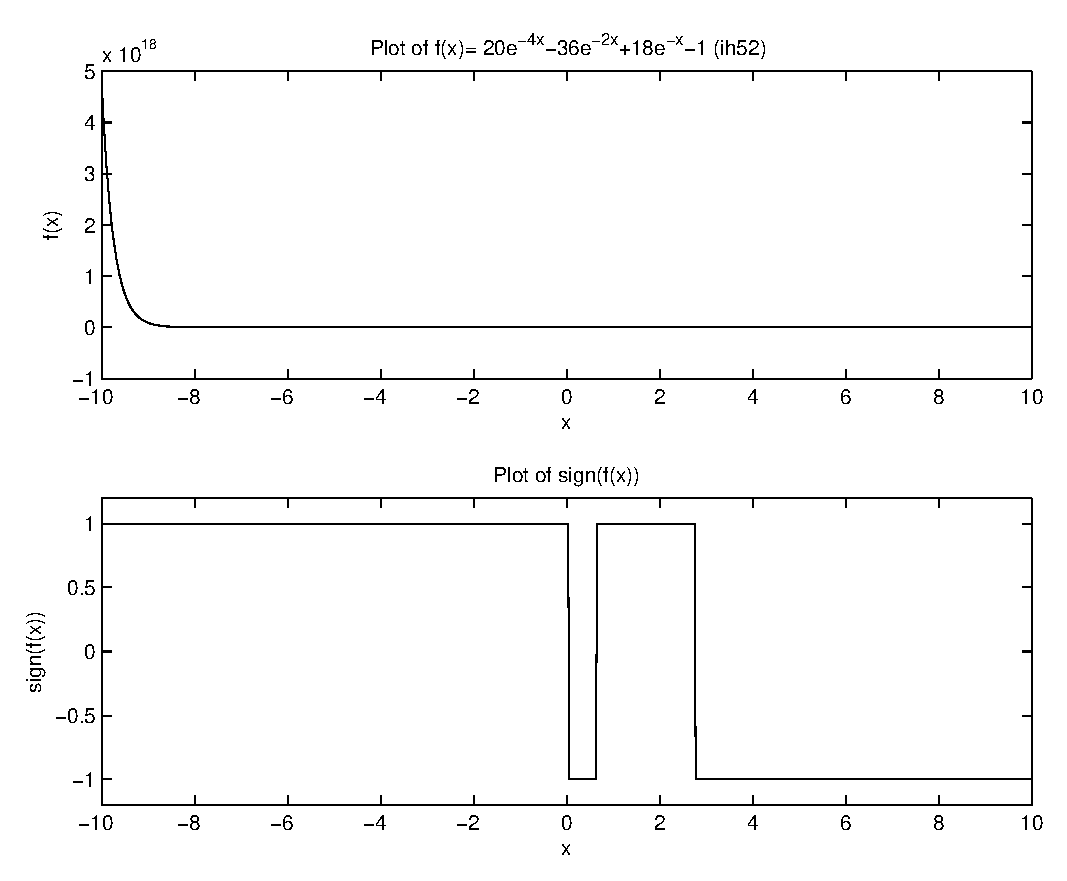
\epsfig{file=F1Plot.eps, width=2.5in} &
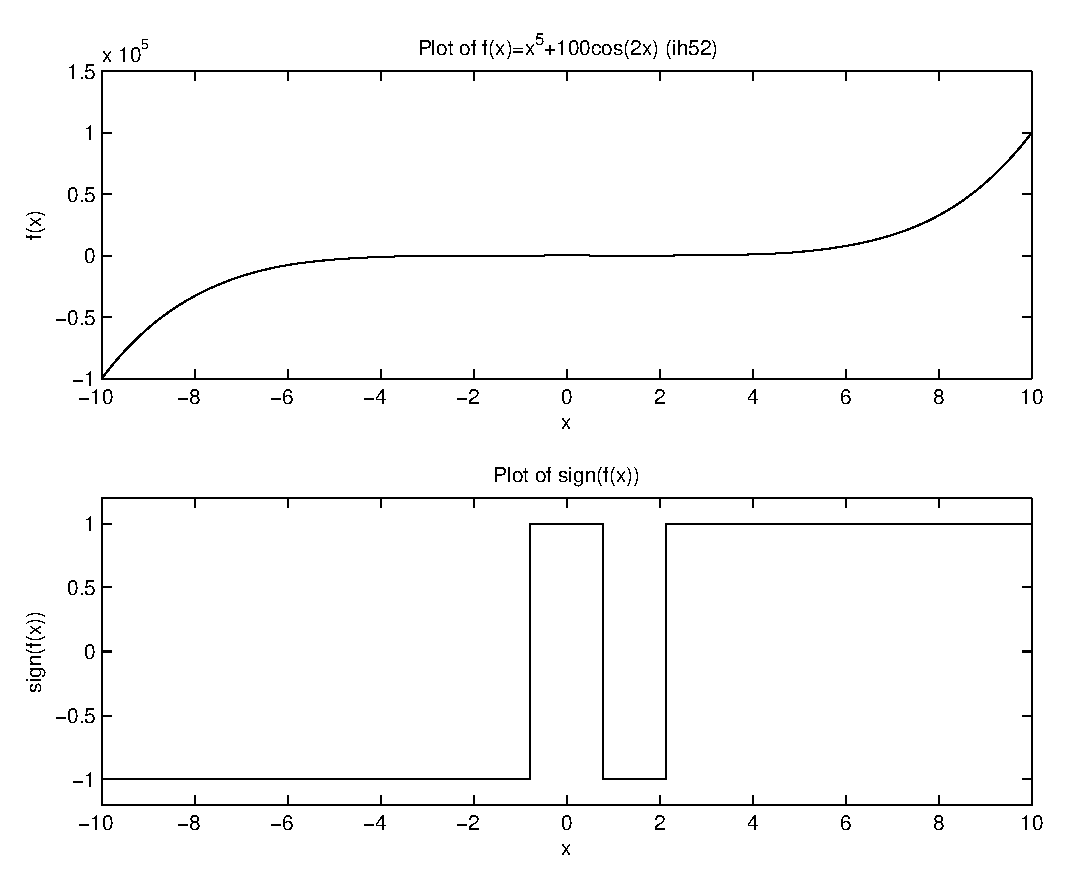
\epsfig{file=F2Plot.eps, width=2.5in}\\
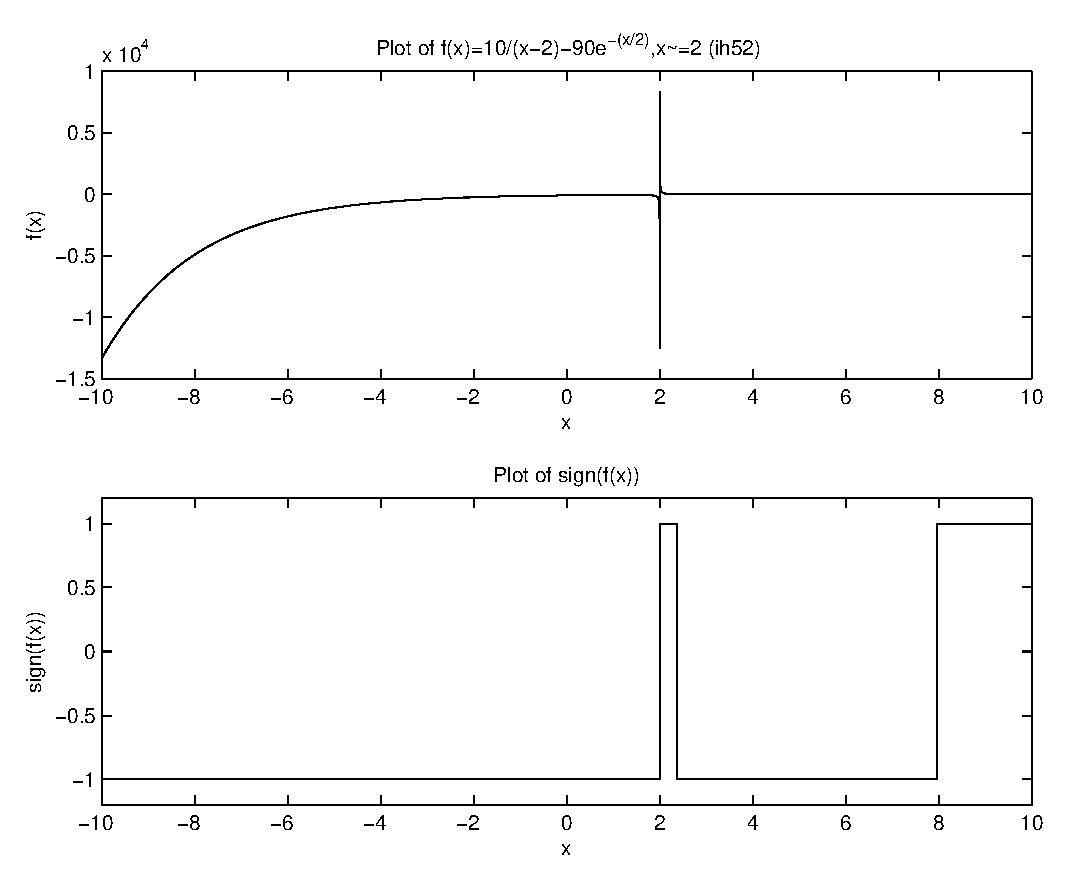
\epsfig{file=F3Plot.eps, width=2.5in} &
~
\end{tabular}
\caption{Basic Roots Problems}
\end{center}
\end{figure}


\begin{figure}[htb!]
\begin{center}
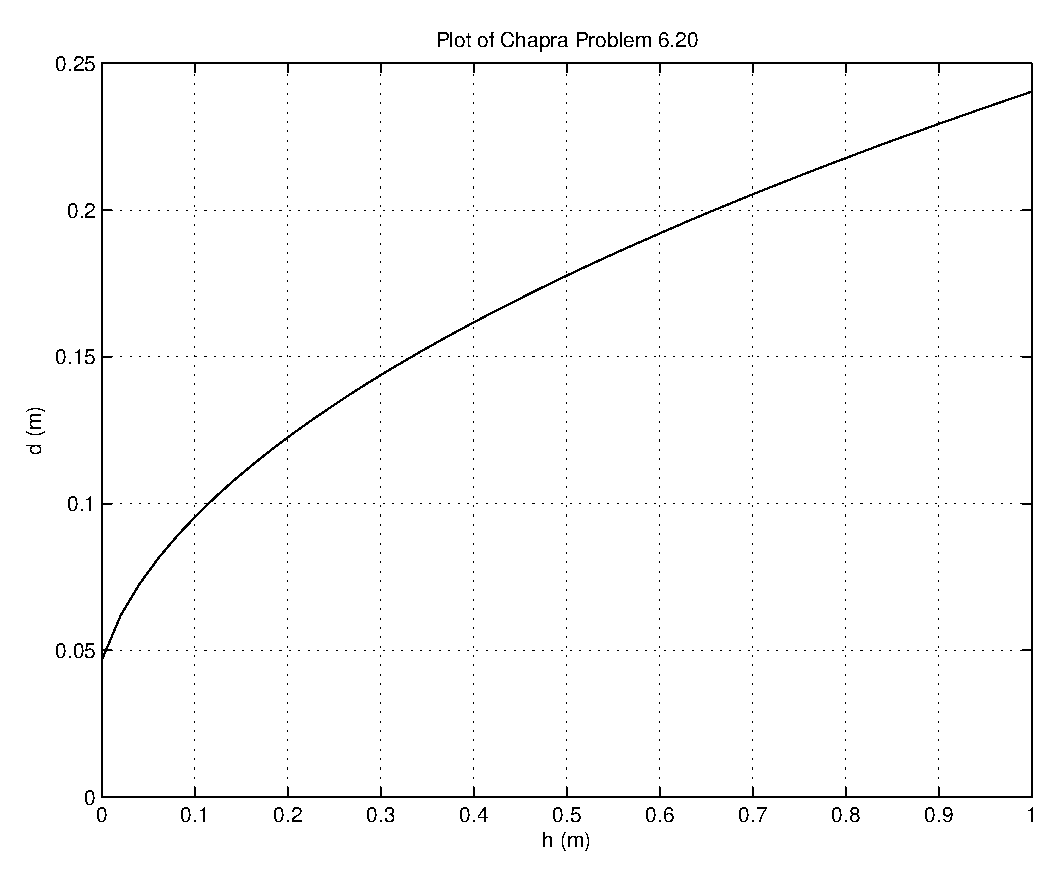
\epsfig{file=Chapra620Fig.eps, width=4in}
\caption{Plot of d vs. h from Chapra 6.20}
\end{center}
\end{figure}

\begin{figure}[htb!]
\begin{center}
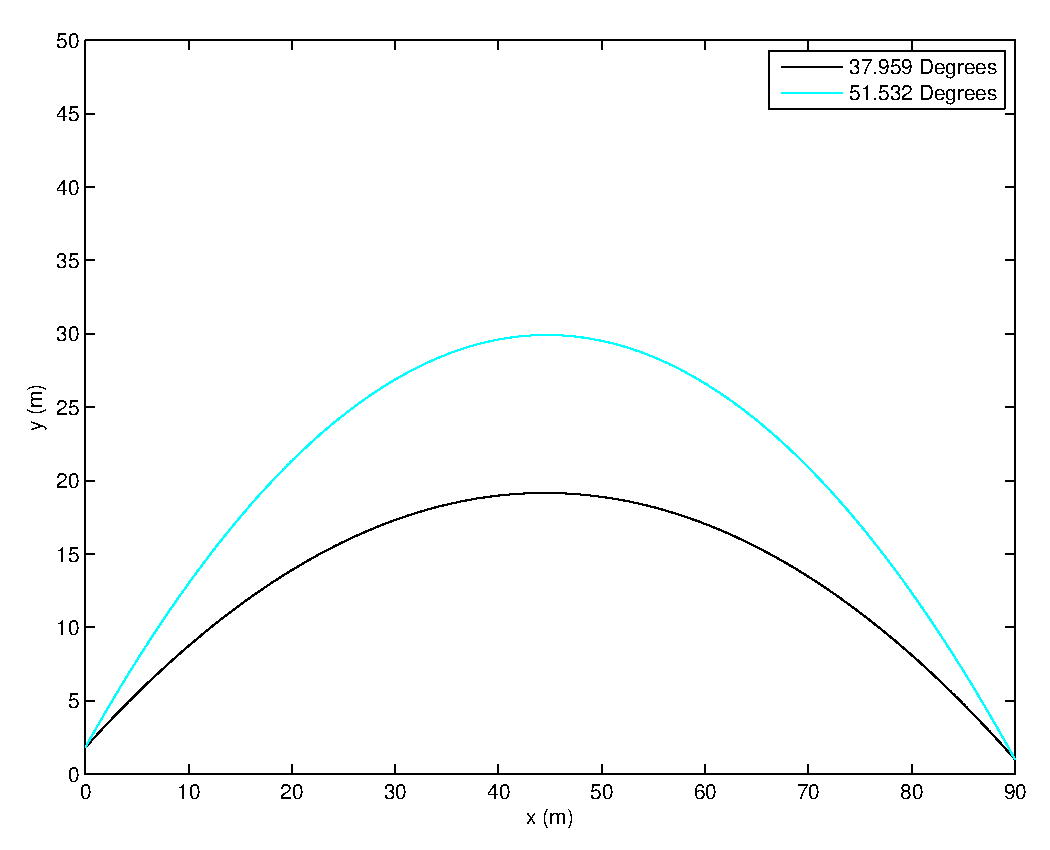
\epsfig{file=Chapra621BballPlot.eps, width=4in}
\caption{Plot of trajectories from Chapra 6.21}
\end{center}
\end{figure}

\begin{figure}[htb!]
\begin{center}
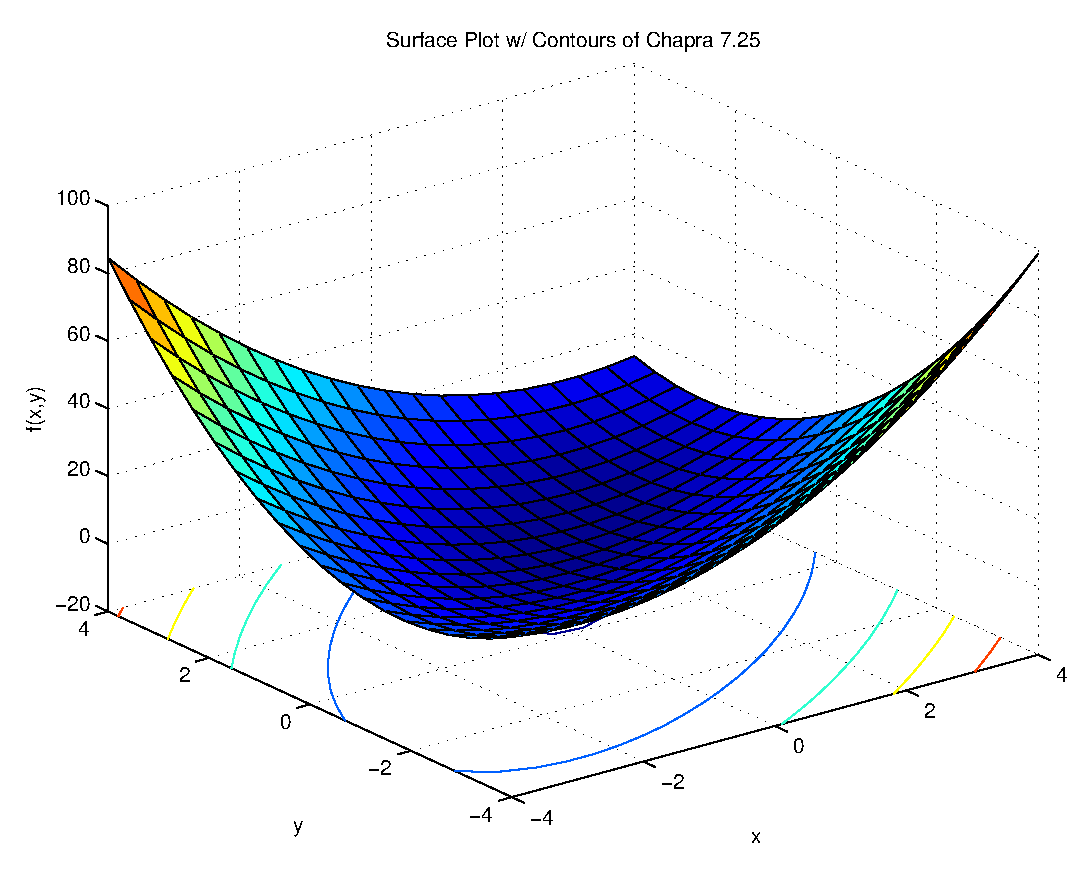
\epsfig{file=Chapra725Plot.eps, width=4in}
\caption{Surface plot with contours of Chapra 7.25}
\end{center}
\end{figure}

\begin{figure}[htb!]
\begin{center}
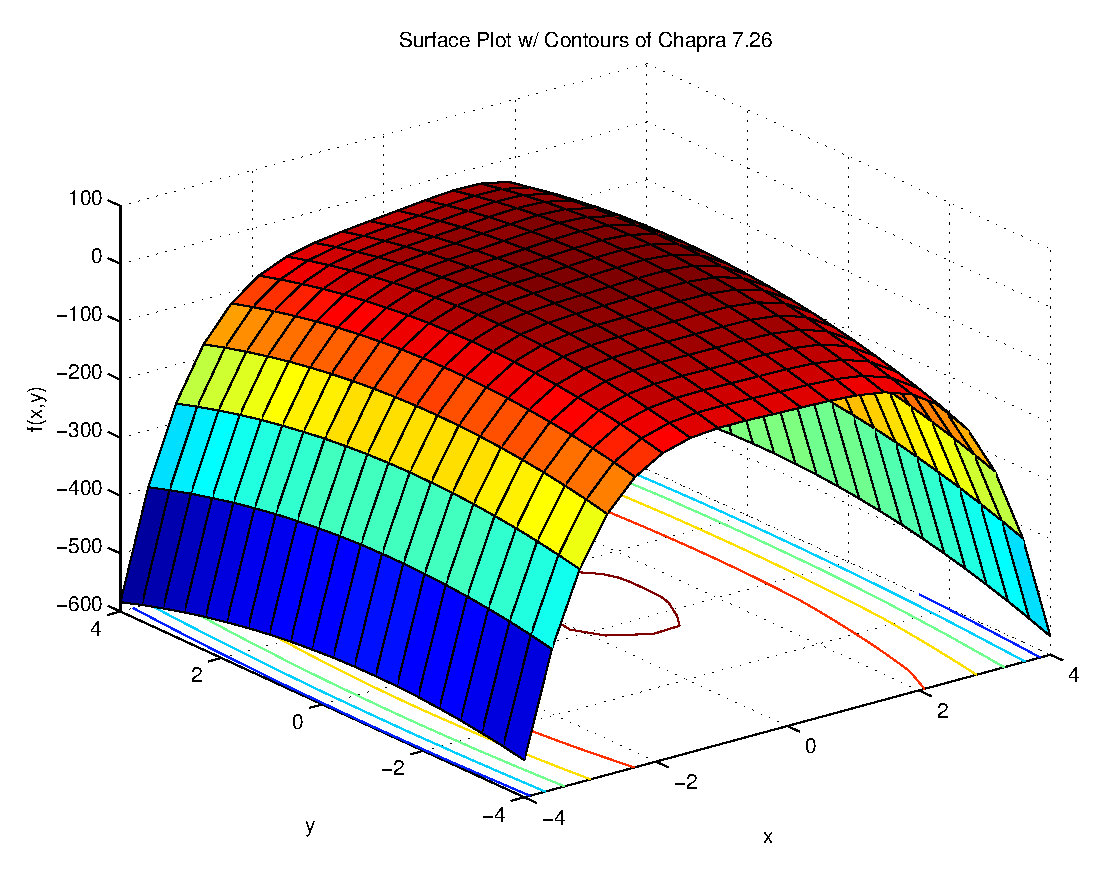
\epsfig{file=Chapra726Plot.eps, width=4in}
\caption{Surface plot with contours of Chapra 7.26}
\end{center}
\end{figure}

\begin{figure}[htb!]
\begin{center}
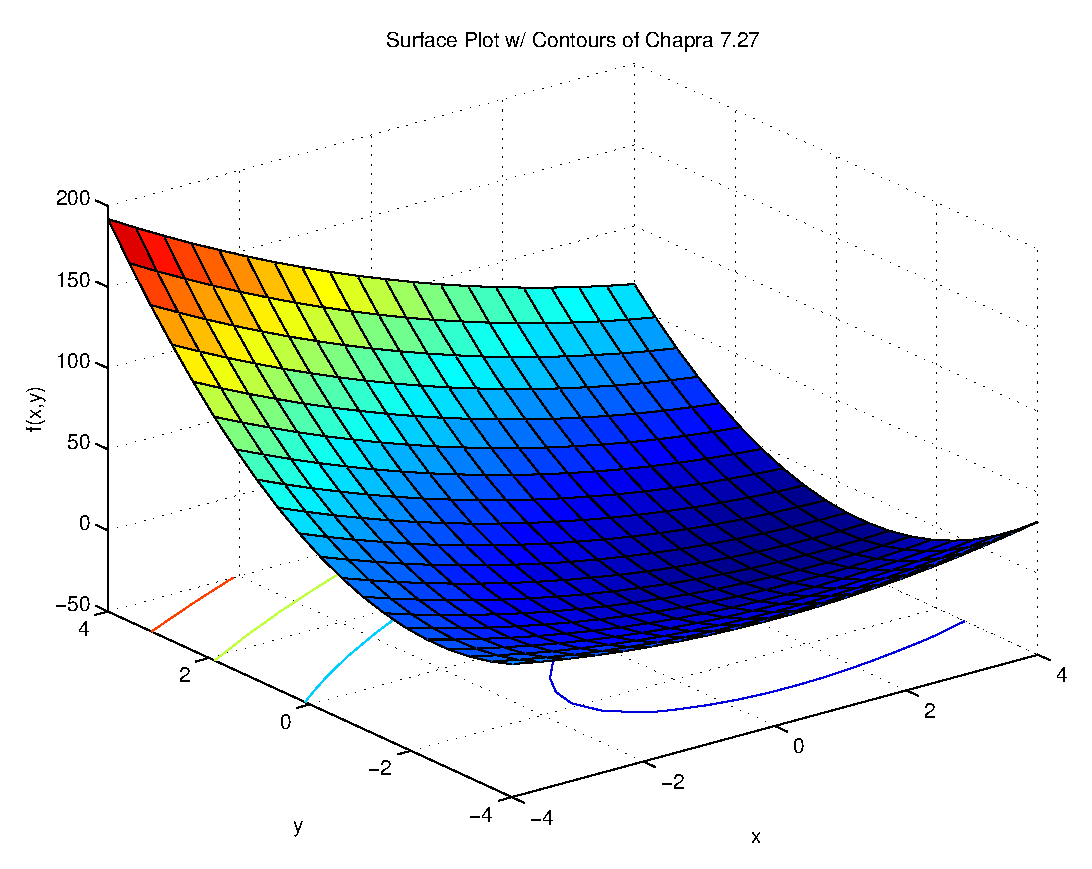
\epsfig{file=Chapra727Plot.eps, width=4in}
\caption{Surface plot with contours of Chapra 7.27}
\end{center}
\end{figure}


\end{document}
